%*****************************************************************************************
%*********************************** Fourth Chapter **************************************
%*****************************************************************************************

\chapter{Lead iodide perovskite thin films}

\graphicspath{{Chapter4/Figures/}}

Spin coating is a simple process that can be used to fabricate thin films on relatively flat substrates. After a solution is deposited, the substrate is accelerated to its desired final spin speed and continues rotating to remove excess solution. As the solvent evaporates the material self-assembles to form a solid film. The process is commonly used in industry as it can controllably produce films $\sim10\,\textnormal{nm} - 100\,\mu$m thick, covering areas with lateral size $\sim10$\,cm. The film thickness and morphology depend on solution concentration, spin speed and substrate preparation. In this Chapter the formation spin coated of C$_{12}$PI and CHPI thin films will be explored.

\section{Spin coating theory}
Although spin coating is experimentally simple, it is complicated to model due to the large number of factors involved. Initially, fluid inertia and surface tension are important as the fluid front spreads out in spiral waves. Evaporation also begins at this point, and a small boundary layer is formed at the liquid-gas interface. At the end of this step a thin and even film forms on the substrate, and fluid inertia is no longer important. In the next phase a balance between viscous and centrifugal forces causes fluid flow and thinning. The boundary layer in the solution gradually gets thicker, and the solute concentration varies throughout the film thickness. Viscosity rises as a result of solvent evaporation, eventually inhibiting further flow. Further fluid loss is caused by solvent evaporation, which dominates thinning in the latter stages, and eventually solute concentration becomes uniform throughout the film. There is also a small atmospheric boundary layer above the solution that can influence heat and mass transfer, as well as exert shear forces at the interface \cite{Meyerhofer1978, VanHardeveld1995, Lawrence1988}. The initial acceleration may also affect final film thickness, as too slow an acceleration can lead to complete solvent evaporation before the final spin speed is reached \cite{Birnie2005}.

Meyerhofer used a model where the solvent evaporation was negligible until the mass loss due to rotational forces fell to the level of the evaporation rate, and calculated that
\begin{equation}
h_f \sim C_0(1-C_0)^{-1/3} \omega^{-2/3} \left( \frac{\eta_0}{\rho_0} \right)^{1/3} e^{-1/3} ~,
\label{Meyehofer}
\end{equation}
where $h_f$ is the final film thickness, $C_0$ the initial solution concentration, $\omega$ the spin speed, $\eta_0$ the initial viscosity, $\rho_0$ the initial solution density, and $e$ the evaporation rate \cite{Meyerhofer1978}. Van Hardeveld used a similar model, except the evaporation was modelled more rigorously in terms of rate of mass transfer at the interface, and calculated that
\begin{equation}
m = C_0 \sqrt[3]{\frac{3 \eta e}{2 \rho {\omega}^2}} ~,
\label{Hardeveld}
\end{equation}
where $m$ is the amount of material deposited in the final film \cite{VanHardeveld1995}. The rate determining step for solvent evaporation was found to be mass transfer in the vapour phase, when the evaporation rate is proportional to ${\omega}^{1/2}$. This relationship has been verified experimentally by both Meyerhofer and van Hardeveld \cite{Meyerhofer1978, VanHardeveld1995} such that $h_f \sim \omega^{-1/2}$. The dependence of the final film thickness on initial solution concentration is more complicated as $\eta_0$ and $\rho_0$ will also depend on concentration. Lawrence's model considered both the solvent and atmospheric boundary layers, and found that
\begin{equation}
h_f \sim C_0 \left(\frac{\eta_0}{\rho_0} D_0 \right)^{1/4} \omega^{-1/2} ~,
\label{Lawrence}
\end{equation}
where $D_0$ is the initial solvent diffusivity \cite{Lawrence1988}.

Taking into account evaporation, all three models above agree that $h_f \sim \omega^{-1/2}$, but experimentally other values have been found \cite{Lawrence1988}. Lawrence indicated that an exponent of $\omega$ less than $-0.5$ may be due to films that had not completed the full spinning process, and was thus thicker than the calculations indicated. Shear thinning, where the viscosity of the solution decreases with an increased shear stress, may also be responsible \cite{Lawrence1988}.

\section{Experimental methods}
\label{sec:glass}
\begin{figure}[h!]
\centering    
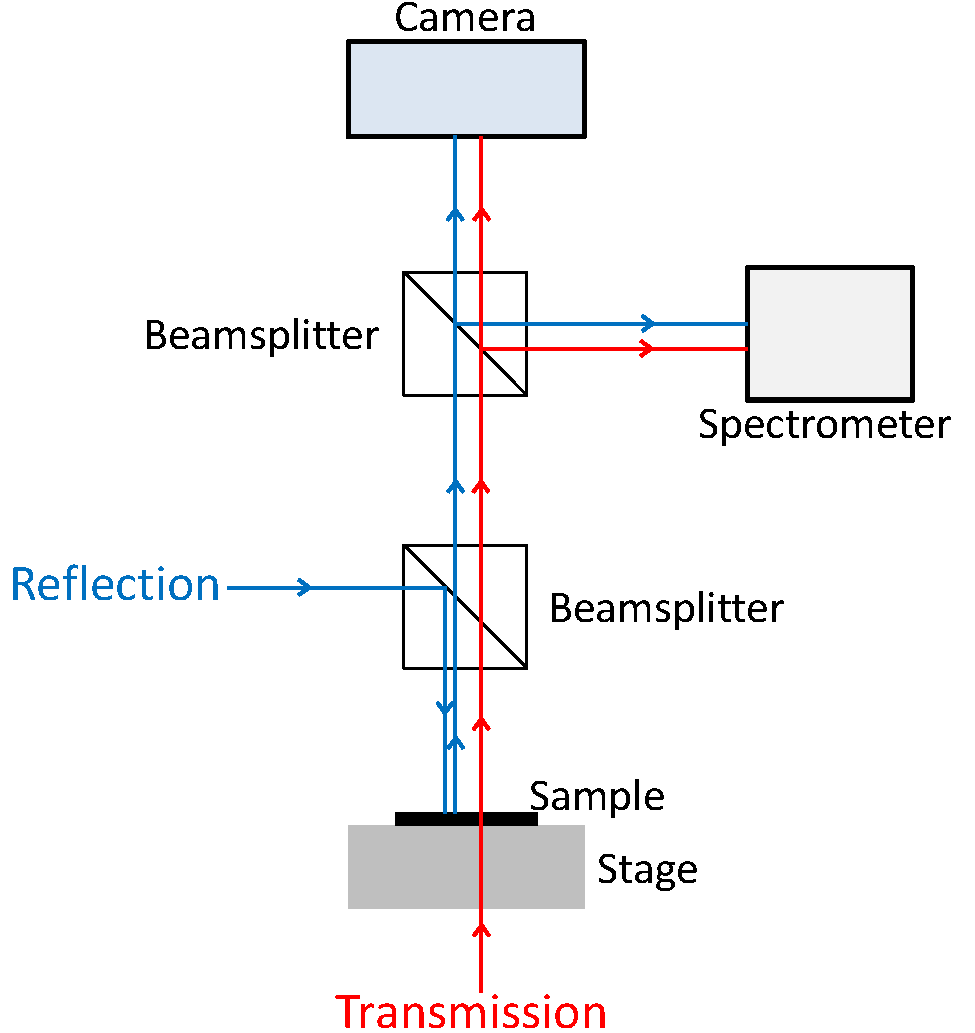
\includegraphics[width=0.6\textwidth]{Microscope}
\caption{Schematic of optical microscopy and spectroscopy setup, including the reflection and transmission beam paths.}
\label{Microscope}
\end{figure}
Spin coating solutions are prepared by dissolving a chemically synthesised perovskite powder [Sec.\,\ref{sec:solutiongrowth}] in tetrahydrofuran (THF) with a concentration of 20\,mg/ml. Silica substrates are sonicated in a four-step process for approximately 15 minutes per solvent: firstly a deionised water and detergent solution, then deionised water, acetone, and finally isopropanol. Three additional substrate preparation techniques are investigated in order to create the most uniform films: (1) \ce{CO2} snowjetting, where a high velocity mix of gaseous and solid carbon dioxide is focused on and substrate, cleaning the surface as a result of the momentum transfer and solvent action of \ce{CO2} \cite{Snowjet}. (2) Silanisation, where substrates are dipped in a 2 vol\% solution of aminopropyltriethoxy silane (APTES) in dry acetone for approximately 90 minutes. A self-assembled monolayer of silane molecules forms on the substrate, and in the case of APTES the surface is functionalised with amine groups. (3) Plasma etching, where substrates are treated using a Diener Electronic Femto plasma system for 5 minutes, using the oxygen plasma to clean contaminants on the substrate. The surface is then functionalised with hydroxyl groups and becomes more hydrophilic. Perovskite films are characterised using optical microscopy and spectroscopy (collected over areas with diameter $\approx 20\,\mu$m unless otherwise specified) [Fig.\,\ref{Microscope}], and the film thickness determined by AFM measurements on scratched areas of the film.

\begin{figure}[h!]
\centering    
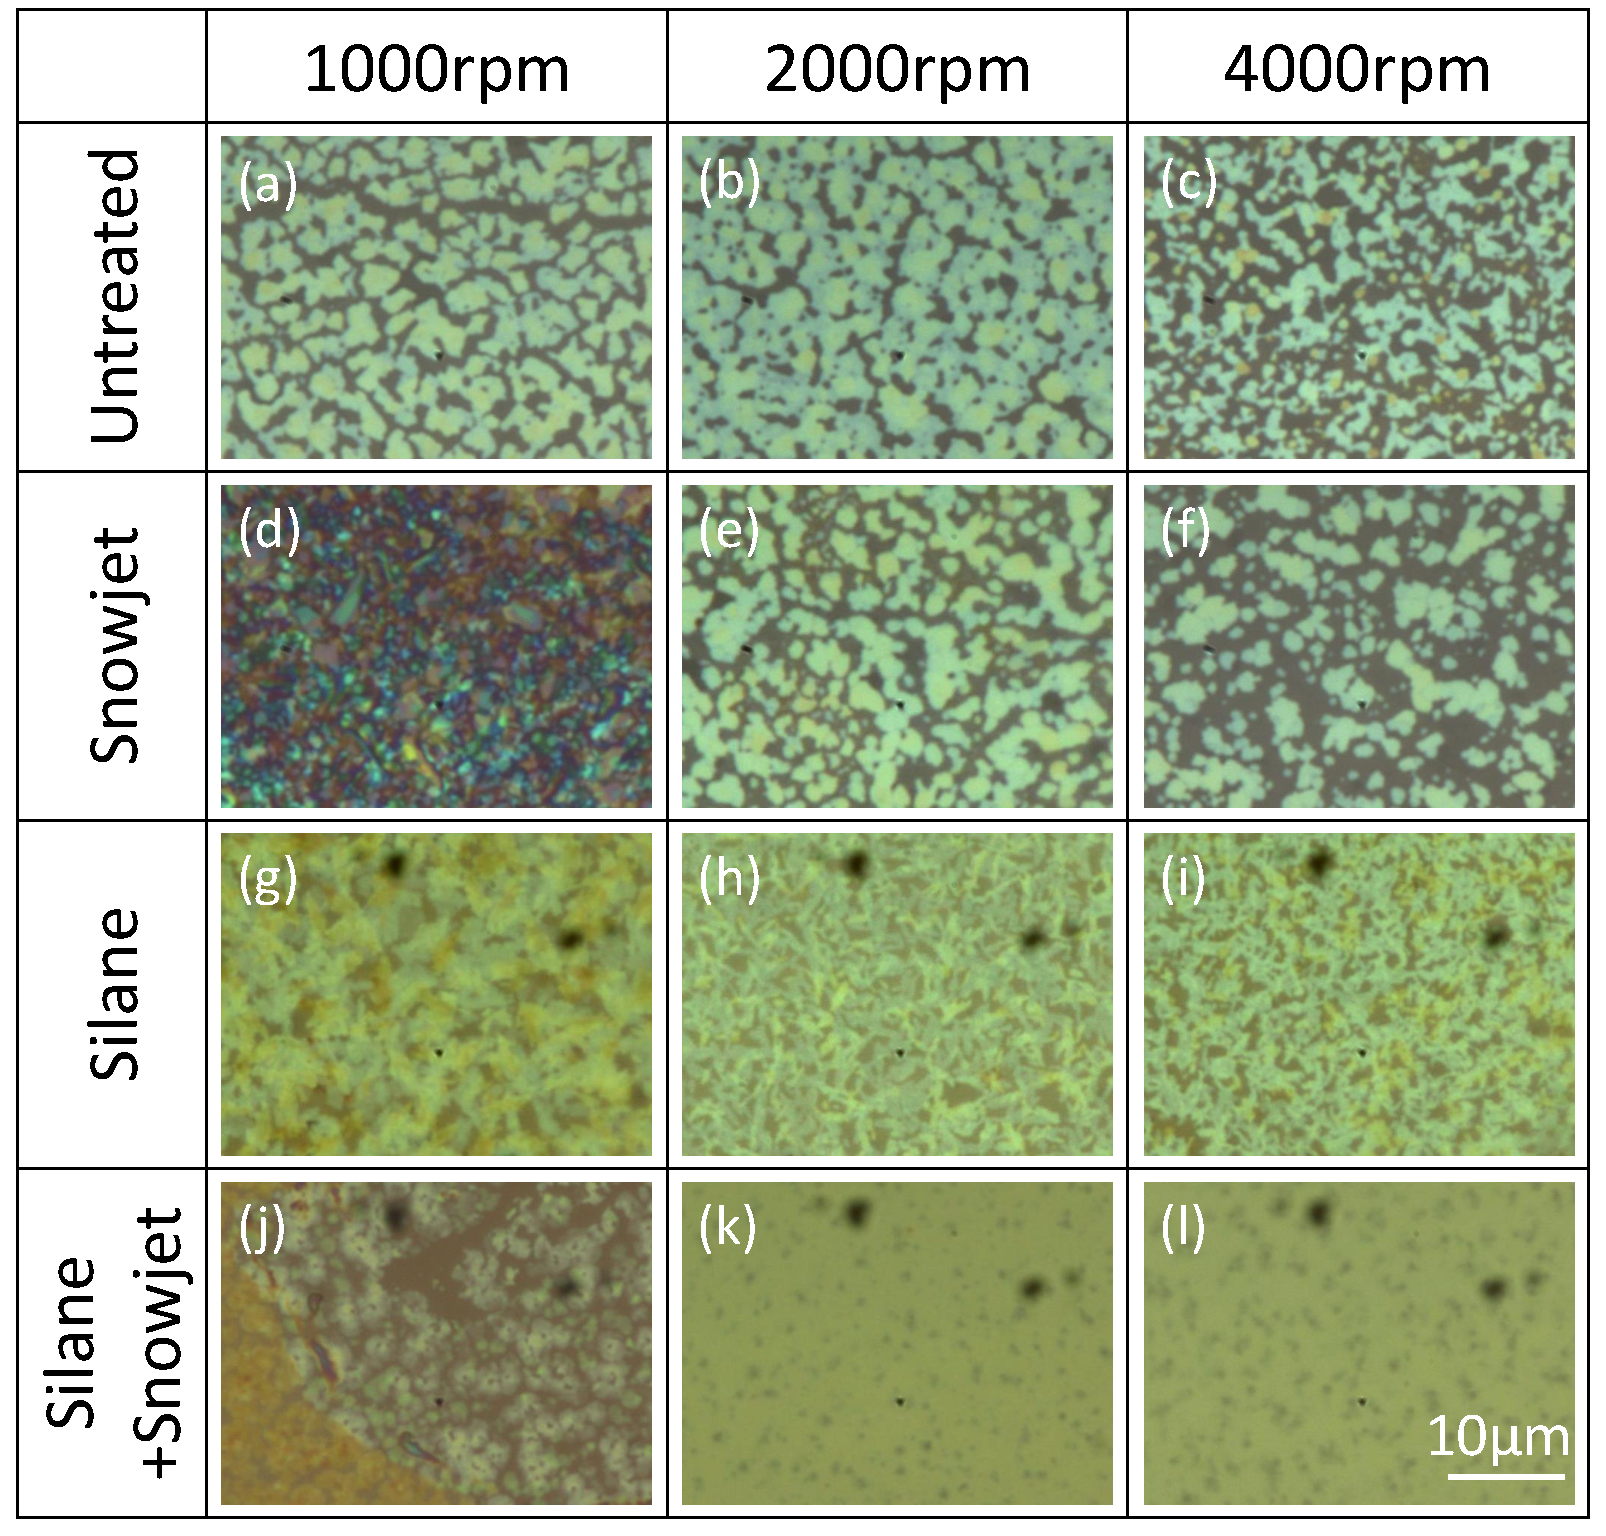
\includegraphics[width=0.88\textwidth]{Fig1}
\caption{BF images at 100$\times$ magnification of spin coated C$_{12}$PI films, with spin speed and substrate preparation as labelled. Note the substrate was heated for (d) only.}
\label{4Fig1}
\end{figure}
\section{C$_{12}$PI thin films}
Bright field (BF) images of C$_{12}$PI films at 100$\times$ magnification are shown in Fig.\,\ref{4Fig1}. Due to the hydrophobic nature of the organic molecule, C$_{12}$PI films show significant dewetting without substrate functionalisation [Figs.\,\ref{4Fig1}(a-f)], and for this reason no films are formed on plasma etched substrates. The non-uniform film in Fig.\,\ref{4Fig1}(d) does not exhibit such dewetting as the substrate was heated before application of the C$_{12}$PI solution, thus the solvent evaporated before excess fluid could be removed. Silanisation increases interactions between constituents of C$_{12}$PI and the substrate, thereby improving film coverage [Figs.\,\ref{4Fig1}(g-i)]. Indeed a further snowjet step removes excess APTES that may have remained after silanisation, reducing surface roughness and producing the most uniform C$_{12}$PI samples [Figs.\,\ref{4Fig1}(k,l)].

\begin{figure}[h!]
\centering
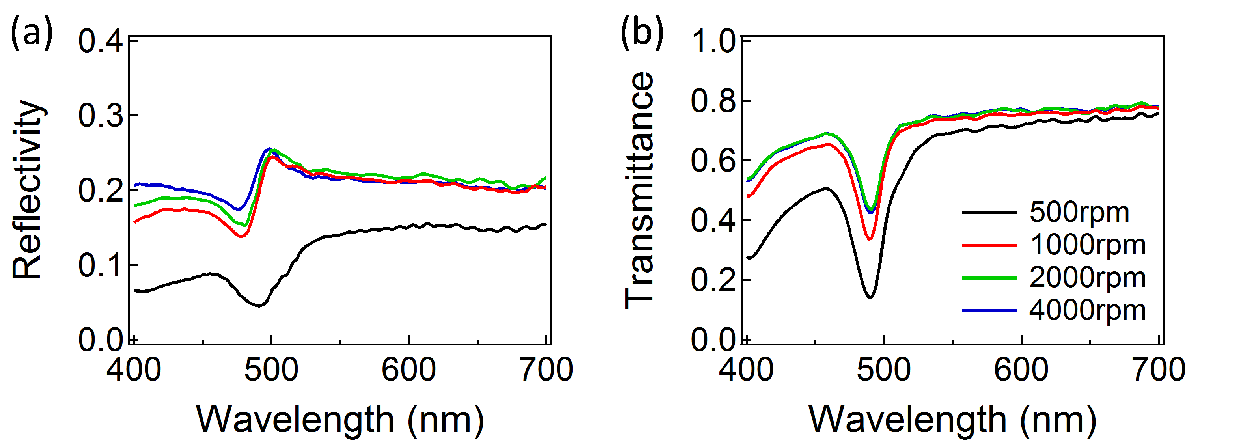
\includegraphics[width=\textwidth]{Fig2}
\caption{(a) Reflection and (b) transmission spectra for C$_{12}$PI films on silanised glass substrates.}
\label{4Fig2}
\end{figure}
\subsection{Spin speed}
Optical spectra of C$_{12}$PI films created on silanised substrates illustrate the general trends observed for all substrate preparations [Fig.\,\ref{4Fig2}]. The exciton appears as a Fano resonance at 490\,nm in reflectivity due to interference between its narrow resonance and the continuum background, while a dip appears in the transmittance spectra. Although both phases of C$_{12}$PI are observed for films below 2000\,rpm [Sec.\,\ref{sec:Cnphases}], here we consider only the high energy exciton. Spectra can be directly correlated to the BF images, hence increased roughness observed in 500\,rpm films translate to a lowering of the overall reflectivity. In the same way, similarities in the morphologies of films made above 1000\,rpm [Figs.\,\ref{4Fig1}(g-i)] lead to almost identical optical spectra. As C$_{12}$PI is a multilayer system, the amplitude of the exciton dip in transmission spectra can be used as a gauge of the film thickness, and from Fig.\,\ref{4Fig2}(b) we see that the film thickness decreases with spin speed as expected.

\begin{figure}[h!]
\centering
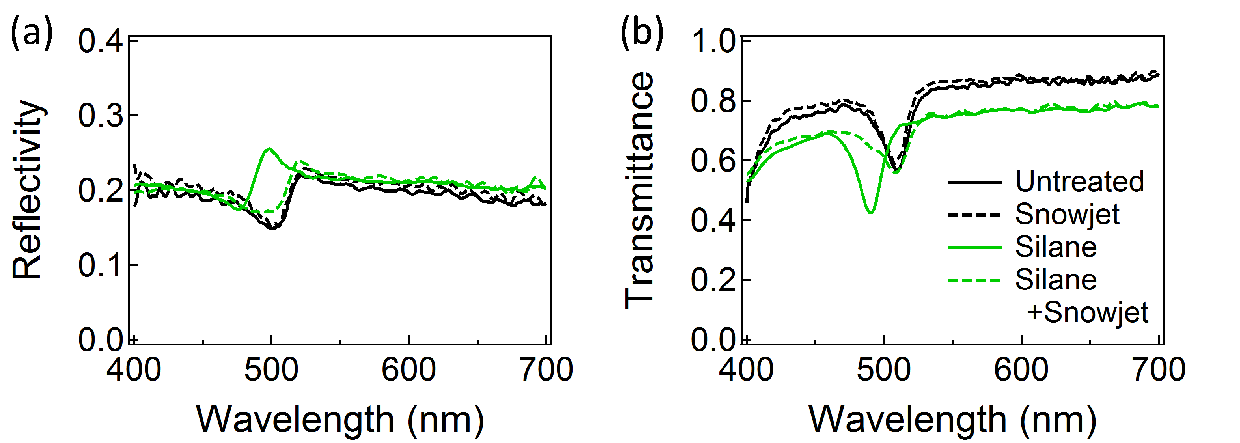
\includegraphics[width=\textwidth]{Fig3}
\caption{(a) Reflection and (b) transmission spectra for 4000\,rpm C$_{12}$PI films.}
\label{4Fig3}
\end{figure}
\subsection{Substrate preparation}
Optical spectra of 4000\,rpm C$_{12}$PI films made using a variety of substrate preparation techniques are shown in Fig.\,\ref{4Fig3}. The reflectivity spectra are almost identical for all substrate preparations [Fig.\,\ref{4Fig3}(a)], with the exception of the silanised substrate where excess APTES molecules led to increased surface roughness, thus favouring the more crumpled and higher energy C$_{12}$PI phase. Removal of the excess silane via snowjetting creates flatter inorganic sheets and lowers the exciton energy. Dewetting of C$_{12}$PI films on non-functionalised substrates produces an increase in the film transmittance away from the exciton resonance [Fig.\,\ref{4Fig3}(b)].

\begin{figure}[h!]
\centering
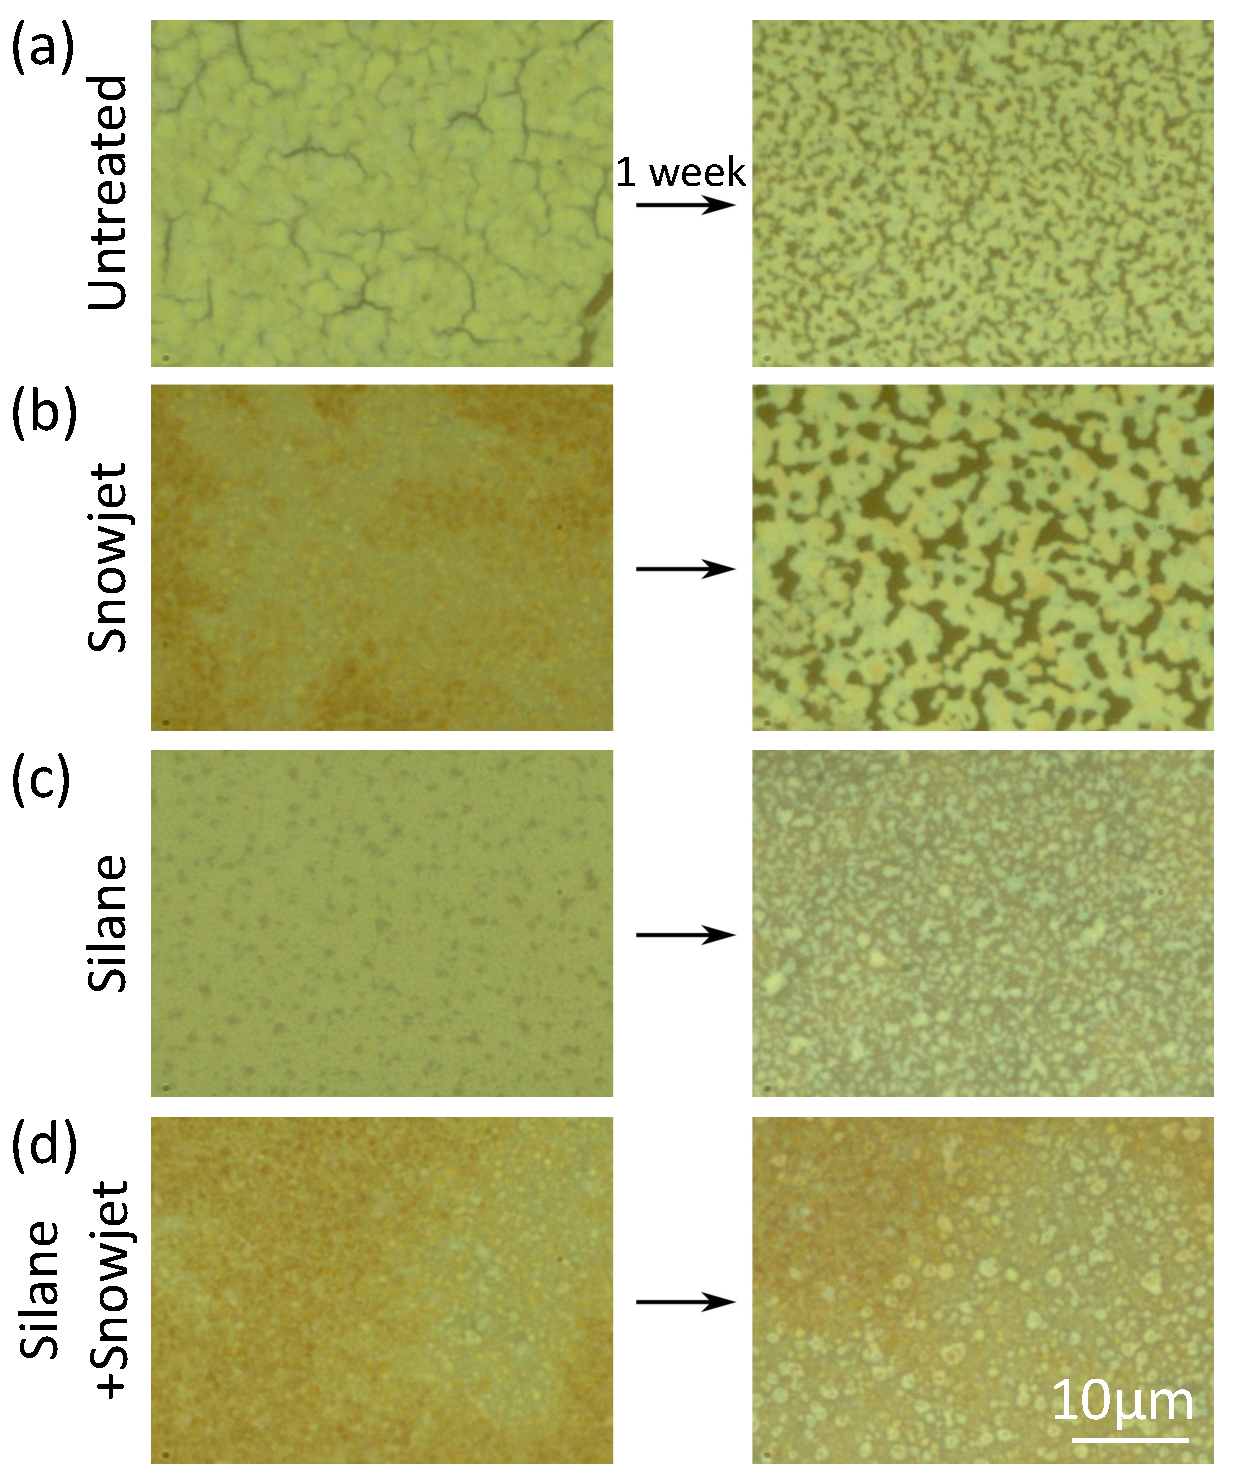
\includegraphics[width=0.65\textwidth]{Fig4}
\caption{Degradation of 2000\,rpm C$_{12}$PI thin films shown in $100\times$ magnification BF images. Images of the sample were taken as-made (left), and after one week in standard conditions (right).}
\label{4Fig4}
\end{figure}
\subsection{Sample degradation}
BF images at 100$\times$ magnification of 2000\,rpm C$_{12}$PI films as-made (left) and after one week in standard conditions (right) are shown in Fig.\,\ref{4Fig4}. All films show signs of dewetting or diffusion, highlighting the importance of placing C$_n$PI films in low humidity atmospheres, or capping with polymer layers to prevent sample degradation \cite{Pradeesh2009}.

\begin{figure}[h!] 
\centering    
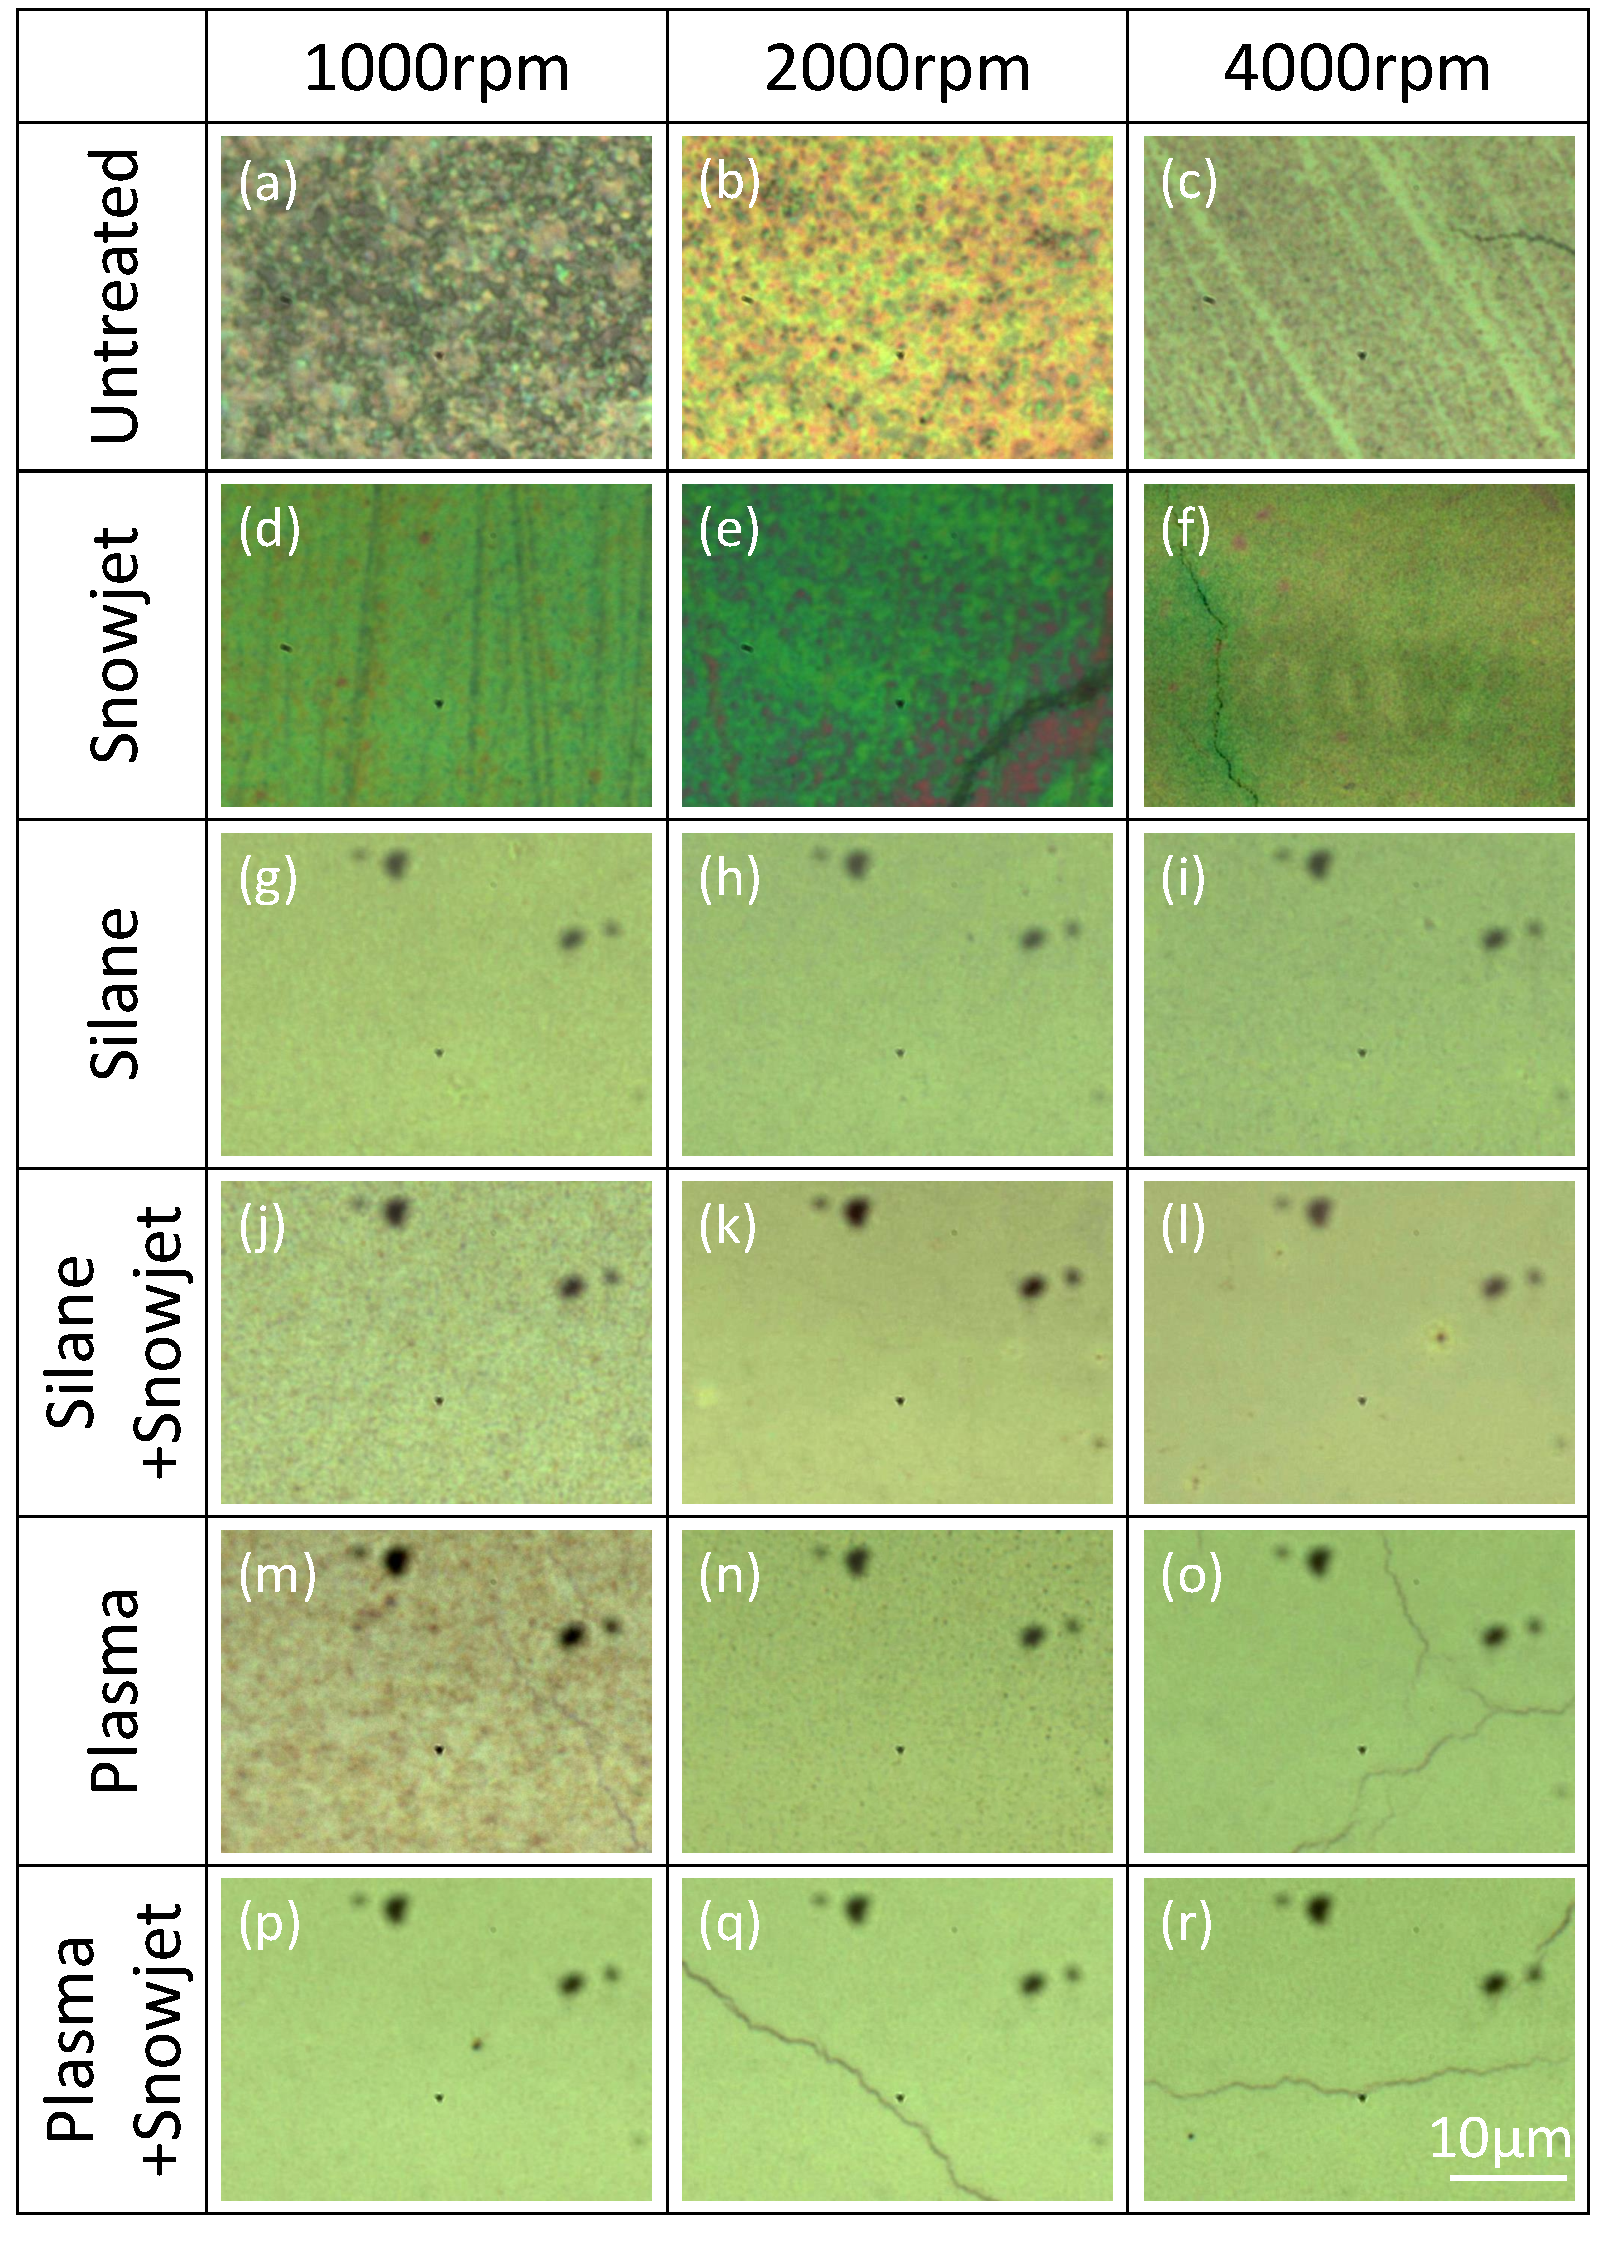
\includegraphics[width=0.9\textwidth]{Fig5}
\caption{BF images at 100$\times$ magnification of spin coated CHPI films, with spin speed and substrate preparation as labelled. The black marks seen on (g-r) are due to dust particles on the microscope lens.}
\label{4Fig5}
\end{figure}
\section{CHPI thin films}
BF images of CHPI films at 100$\times$ magnification are shown in Fig.\,\ref{4Fig5}. No dewetting is observed with CHPI due to increased hydrophilicity of the organic molecule. Both snowjetting and high spin speeds improved the uniformity of samples [Figs.\,\ref{4Fig5}(a-f)], however the best films are produced with silanised substrates, regardless of spin speed [Figs.\,\ref{4Fig5}(g-l)]. A similar effect is seen in plasma etched substrates [Figs.\,\ref{4Fig5}(m-r)].

\subsection{Spin speed}
\begin{figure}[h!] 
\centering    
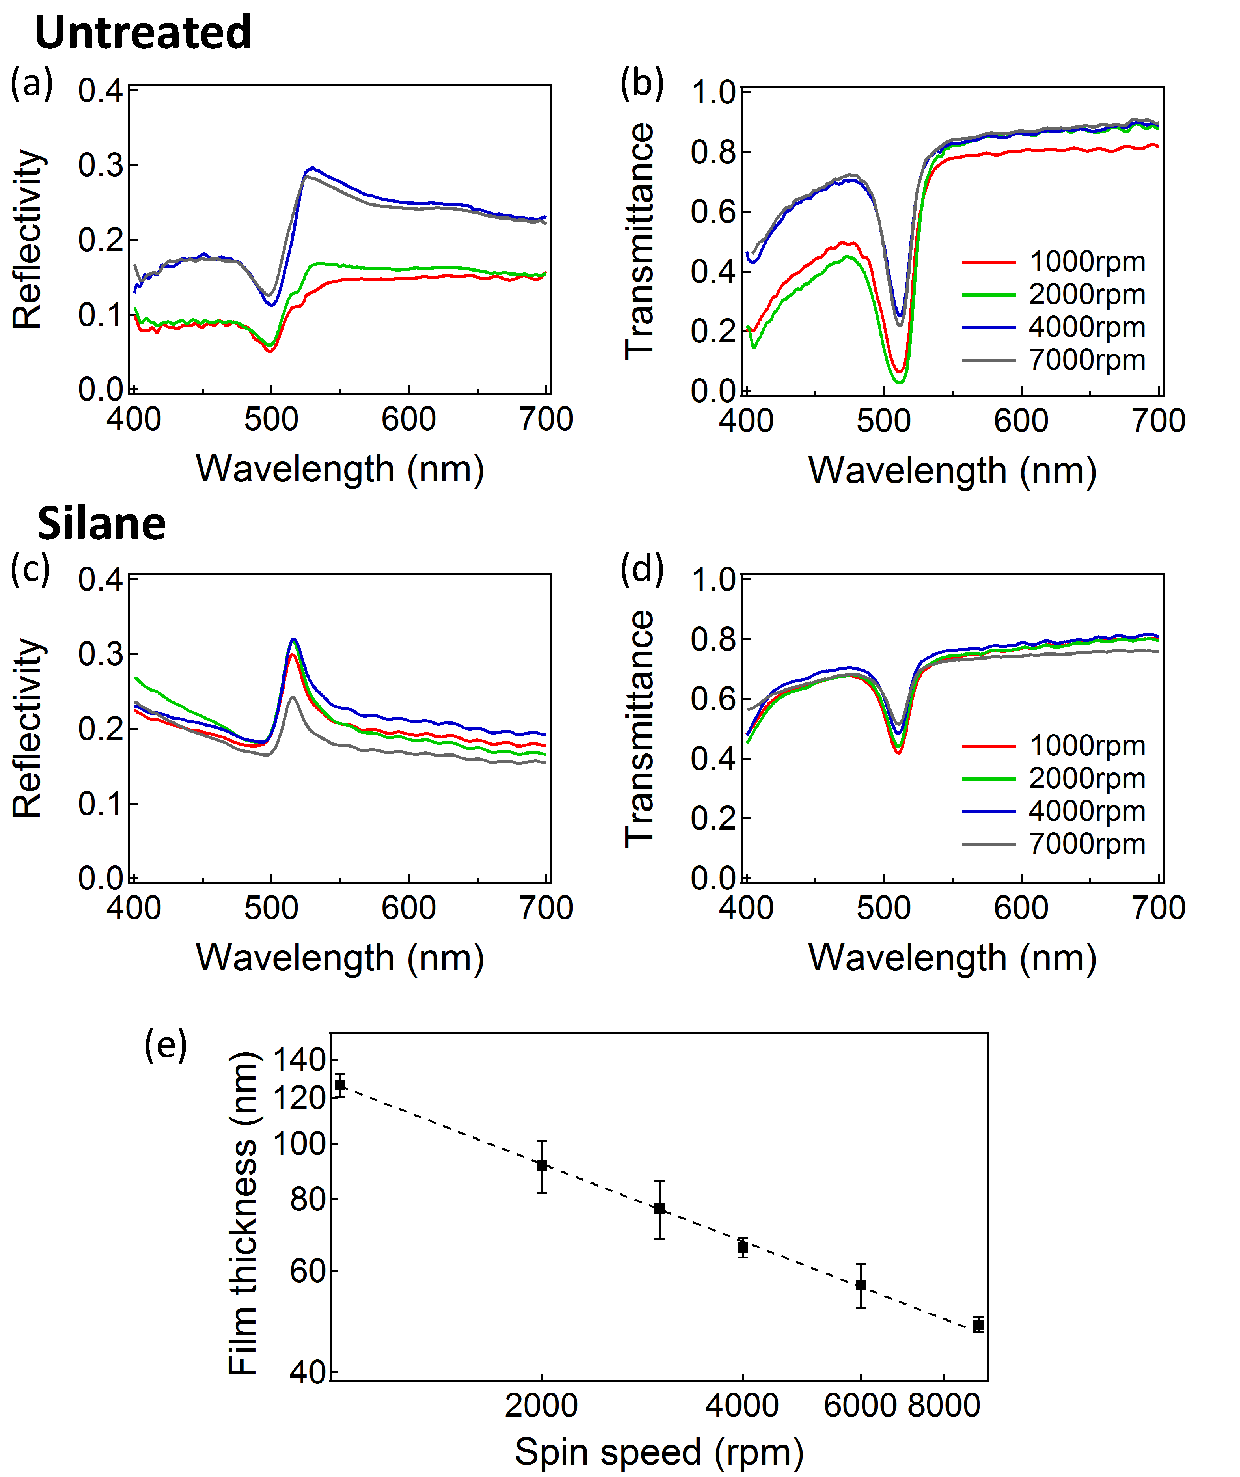
\includegraphics[width=\textwidth]{Fig6}
\caption{Reflection and transmission spectra for CHPI films prepared on (a,b) untreated and (c,d) silanised substrates. (e) Effect of spin speed on CHPI film thickness on untreated substrates for 30\,mg/ml solutions. The dashed lines represents a fit to $a\omega^{-b}$, with $b=0.45\pm0.01$.}
\label{4Fig6}
\end{figure}
Optical spectra of CHPI films created on untreated or silanised substrates are shown in Fig.\,\ref{4Fig6}, with the exciton resonance at 506\,nm. For untreated substrates, noticeable differences in the spectra between 2000 and 4000\,rpm films are caused by a morphology change: at low spin speeds increased film roughness produces lower overall reflectivity, and the appearance of a higher energy exciton leads to an apparent increase in the linewidth of the transmission dip [Figs.\,\ref{4Fig6}(a,b)]. Such extra resonances have been observed in thick perovskite films ($>120$\,nm) and are attributed to stacking faults, strain and structural misalignment in the structure \cite{VijayaPrakash2009}. In contrast, as expected from their BF images [Fig.\,\ref{4Fig5}(g-i)] the spectra for silanised substrates exhibit the same features at all spin speeds [Figs.\,\ref{4Fig6}(c,d)], the main difference being a change in the amplitude of the exciton resonance as a result of the film thickness. Film thickness measurements for around 10 films made using untreated substrates can be fit to $a\omega^{-b}$ with $b=0.45\pm0.01$ [Fig.\,\ref{4Fig6}(e)], close to the $\omega^{-0.5}$ relationship predicted by theory. Although this discrepancy may be attributed to the somewhat simplified model, a larger source of error comes from AFM measurements of film thickness. It can be difficult to provide accurate values due to film/substrate roughness, or small gradients in the film thickness. These effects are hard to quantify and not represented in Fig.\,\ref{4Fig6}(e), where the error bars are calculated from statistical analysis of the data recorded.

\begin{figure}[] 
\centering    
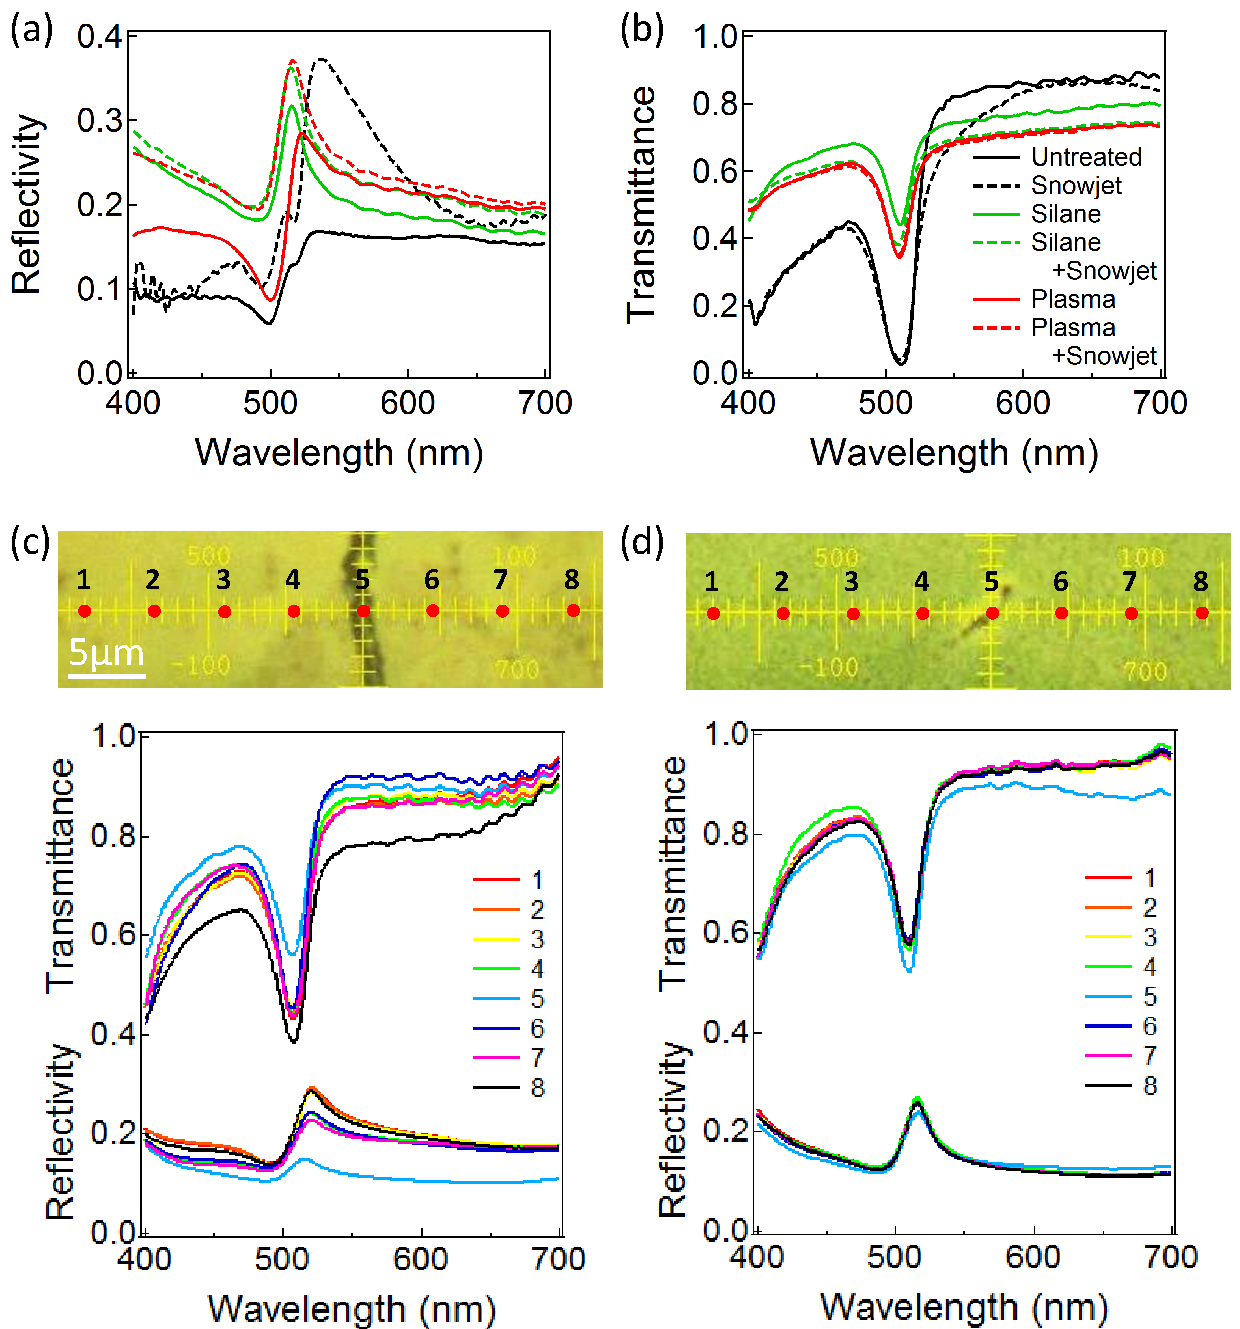
\includegraphics[width=\textwidth]{Fig7}
\caption{((a) Reflection and (b) transmission spectra (collected over areas with diameter $\approx 20\,\mu$m) of 2000\,rpm CHPI films. Reflection and transmission spectra (diameter $\approx1\,\mu$m) of 4000rpm CHPI films prepared on (c) untreated and (d) silanised and snowjetted substrates at the indicated positions.}
\label{4Fig7}
\end{figure}
\subsection{Substrate preparation}
Optical spectra of 2000\,rpm CHPI films made using a variety of substrate preparation techniques are shown in Fig.\,\ref{4Fig7}. The appearance of a second exciton due to structural misalignment is seen in both untreated and snowjetted films. As indicated by their BF images [Fig.\,\ref{4Fig5}(h,k,n,q)], the spectra and morphologies of films made using other substrate preparations are very similar, and the uniformity is greatly improved by functionalisation of the substrate via silanisation or plasma etching. As an indication of the sample uniformity, line scans were made on 4000\,rpm films made using untreated [Fig.\,\ref{4Fig7}(c)], and silanised and snowjetted [Fig.\,\ref{4Fig7}(d)] substrates (over areas with diameter $\approx1\,\mu$m). The near-identical spectra of all areas on the functionalised substrate is further proof of the film uniformity observed in BF images.

\begin{figure}[] 
\centering    
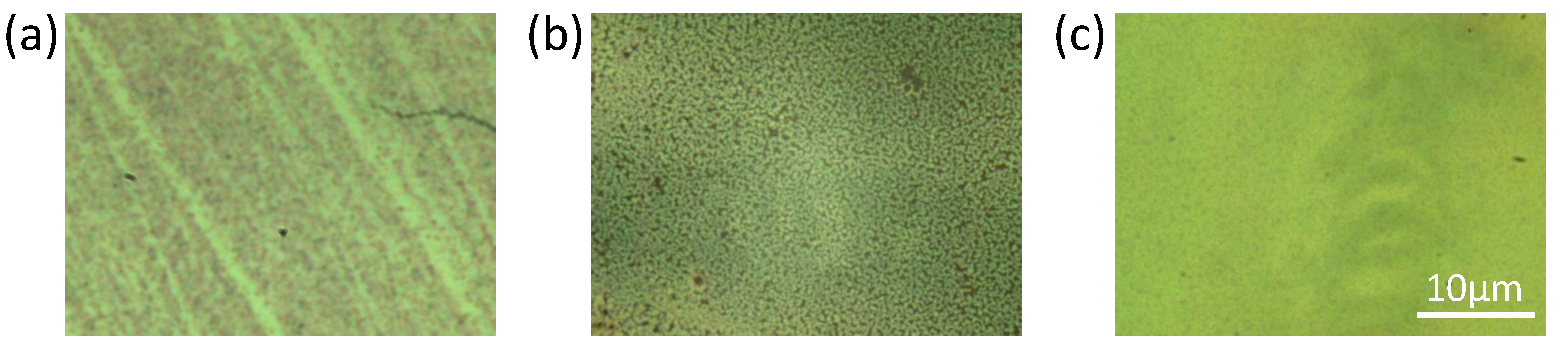
\includegraphics[width=0.85\textwidth]{Fig8}
\caption{BF images at 100$\times$ magnification for 4000\,rpm CHPI films made on untreated substrates in (a) low, (b) high and (c) dehydrated spin coater atmospheres.}
\label{4Fig8}
\end{figure}
\subsection{Humidity}
Hydrogen bonding between the organic and inorganic constituents is essential to assembly of the perovskite structure, therefore unwanted bonding or screening due to water molecules in the atmosphere can disrupt this process. A continuous CHPI film is formed at 4000\,rpm on an untreated substrate in a low humidity atmosphere [Fig.\,\ref{4Fig8}(a)], however the same spin coating conditions lead to dewetting at high humidity despite the hydrophilic organic group [Fig.\,\ref{4Fig8}(b)]. Clearly the spin coater should be desiccated as much as possible in the ideal case, and in order to achieve this the dehydration agent \ce{CaCl2} is placed in the spin coater roughly one hour before film production. The spin coater is also pumped with \ce{N2} gas just before spinning, and the resulting film is very uniform even without the use of substrate functionalisation [Fig.\,\ref{4Fig8}(c)].


\section{Conclusions}
Thin films of PbI perovskites with thickness $30-150$\,nm can be produced reliably using spin coating. Film morphology depends strongly on the organic molecule used in the perovskite, and dewetted films are produced for hydrophobic moieties. However film coverage and uniformity can be improved by using higher spin speeds, or substrate functionalisation techniques such as silanisation. Film thickness is controlled by the spin speed and initial solution concentration, and follows an $\omega^{-0.45}$ dependence, close to theoretical predictions. Formation of the perovskite structure can be disrupted by water in the atmosphere, and a dehydration agent should be placed in the spin coater to controllably produce a low humidity environment. The simplicity and adaptability of spin coating allows PbI perovskite thin films to be deposited on suitable substrates in order to create hybrid nanostructures.